\chapter{Tips and Tricks}
\label{chap:Tips and Tricks}

This chapter handle some of the functions, which provides by Enterprise Architect(EA).
At the first side they seem to be somehow hidden or easy but these simple functions will help you to deal with EA faster and more enjoable.

\section{How to layout elements}

\begin{enumerate}
\item[$\blacktriangleright$]Select a group of elements by drawing a selection box around them all (or select them one by one by holding down \texttt{Ctrl} and clicking on each element).

\item[$\blacktriangleright$]At the right side of last selected element appeared a special Symbol (Fig.~\ref{fig_layout01}).
Click on this symbol to see different possibilities, which you can use to change the appearance of all selected elements of a group simultaneously.
 
 \begin{figure}[htbp]
\begin{center}
  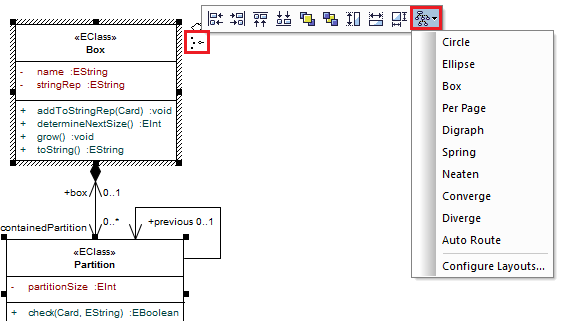
\includegraphics[width=0.5\textwidth]{pics/tricks/layoutElements/layoutElements1}
  \caption{How to layout elements}  
  \label{fig_layout01}
\end{center}
\end{figure}
 
\end{enumerate}


Another way to change the element in the Group is to select them and subsequently, right-click on one of the selected elements.  
Here you can see more functions provided for selected elements, For example ``Align'' (Fig.~\ref{fig_layout02}).
 
 \begin{figure}[htbp]
\begin{center}
  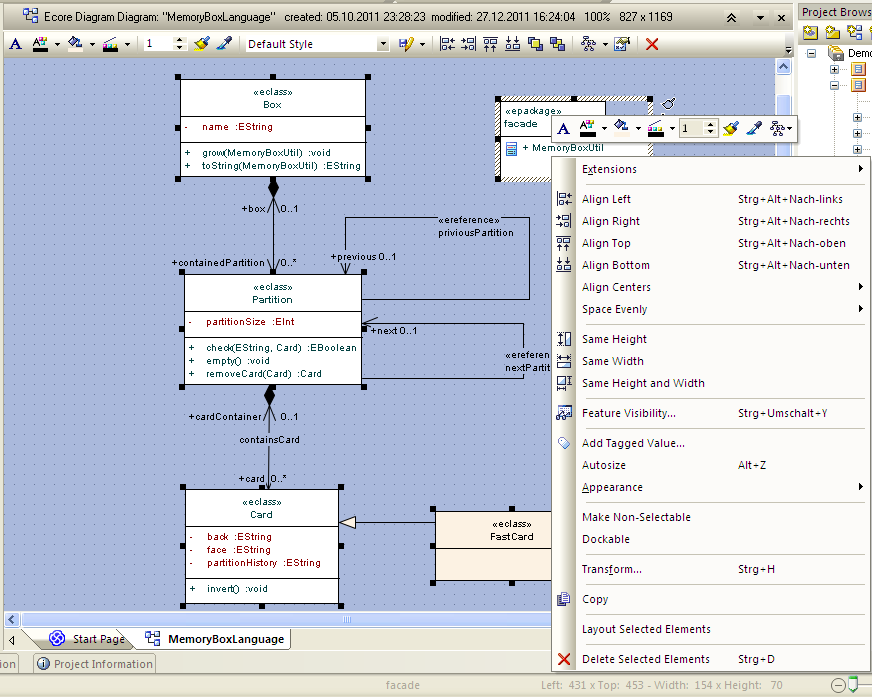
\includegraphics[width=0.5\textwidth]{pics/tricks/layoutElements/layoutElements2}
  \caption{Another way to layout elements}  
  \label{fig_layout02} 
\end{center}
\end{figure}


\section{How to bend lines}
\begin{enumerate}
\item[$\blacktriangleright$]By holding down \texttt{Ctrl} and clicking on each line you can create more points helping bending the lines (Fig.~\ref{fig_bendLine01}).
 
\begin{figure}[htbp]
\begin{center}
  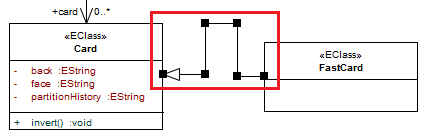
\includegraphics[width=0.5\textwidth]{pics/tricks/bendLine/bendLine1}
  \caption{How to bend lines}   
  \label{fig_bendLine01}
\end{center}
\end{figure}

\item[$blacktriangleright$] You can go back to the previouse form again just by
holding down \texttt{Ctrl} and clicking on each points.
\end{enumerate}

\section{How deleting in EA works (Del vs. Del + Ctrl) }
One of the most common mistakes of users is to delete an element just by 
pressing \texttt{Del}.   
If you delete an element in a diagram just by clicking
\texttt{Del} (Fig.~\ref{fig_DelVsCtrlDel01}), you have delete it just from a diagram
but \emph{not} from \texttt{ProjectBrowser} (Fig.~\ref{fig_DelVsCtrlDel02}).

\begin{figure}[htbp]
\begin{center}
  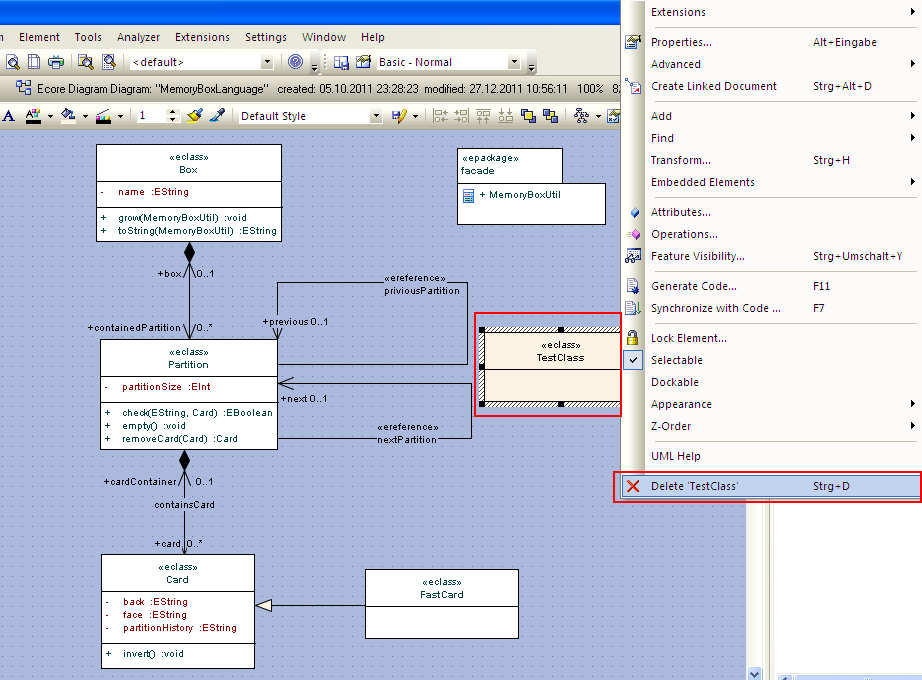
\includegraphics[width=0.5\textwidth]{pics/tricks/DelVsCtrlDel/DelVsCtrlDel1}
  \caption{Deleting a project by clicking Del}  
  
    \label{fig_DelVsCtrlDel01}
\end{center}
\end{figure}  

\begin{figure}[htbp]
\begin{center}
  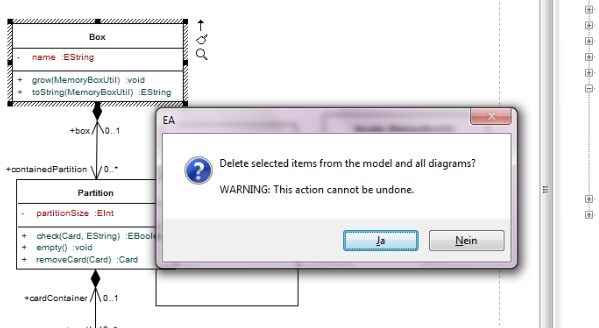
\includegraphics[width=0.5\textwidth]{pics/tricks/DelVsCtrlDel/DelVsCtrlDel2}
  \caption{Deleted element in Project Browser}  
  \label{fig_DelVsCtrlDel02}
\end{center}
\end{figure}  

\begin{enumerate}

\item[$blacktriangleright$] By pressing \texttt{Ctrl+Del} you can delete it
completely from digramm as well as from \texttt{Project Browser}. If you delelte in this way you will see the dialogue
that asked if you want to delete it from model and diagram (Fig.~\ref{fig_DelVsCtrlDel03}).



\begin{figure}[htbp]
\begin{center}
  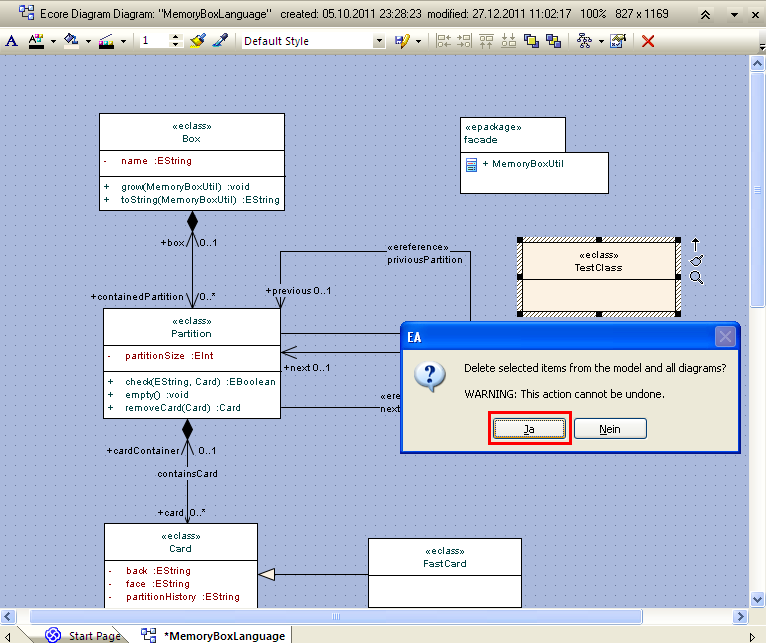
\includegraphics[width=0.5\textwidth]{pics/tricks/DelVsCtrlDel/DelVsCtrlDel3.png}
  \caption{Deleteing a project completely}  
  \label{fig_DelVsCtrlDel03}
\end{center}
\end{figure}  

\end{enumerate}

\section{Using Moflon::Export to ignore projects when exporting}
If you have package, that do not to be exported. You can achieve this by
setting the value of Tagged Values of
Project (Fig.~\ref{fig_ignoreExportingProject01}).

\begin{enumerate}
\item[$\blacktriangleright$]Select “Veiw/Tagged Values” from tool bar.
\begin{figure}[htbp]
\begin{center}
  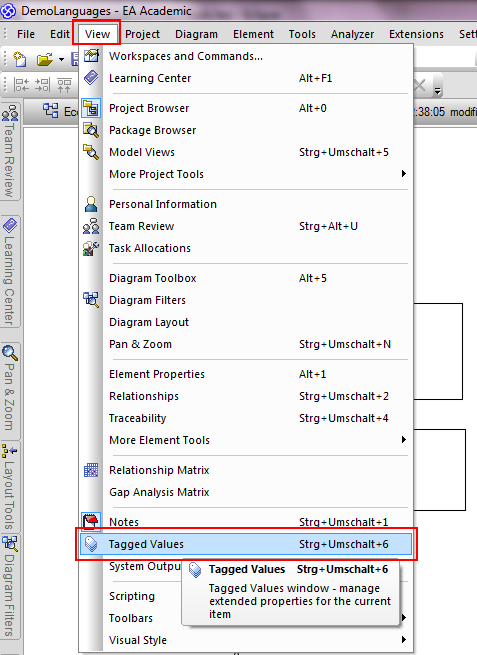
\includegraphics[width=0.5\textwidth]{pics/tricks/ignoreExportingProject/ignoreExportingProject1}
  \caption{view the TaggedValue}  
  \label{fig_ignoreExportingProject01}
\end{center}
\end{figure} 


\end{enumerate}


\begin{enumerate}

\item[$\blacktriangleright$]The default Tagged value is
true(Fig.~\ref{fig_ignoreExportingProject02}). If you want the project to be 
ignored during exporting you have to change the value of ``Moflon::Export'' to
\emph{false} (Fig.~\ref{fig_ignoreExportingProject03}).

\begin{figure}[htbp]
\begin{center}
  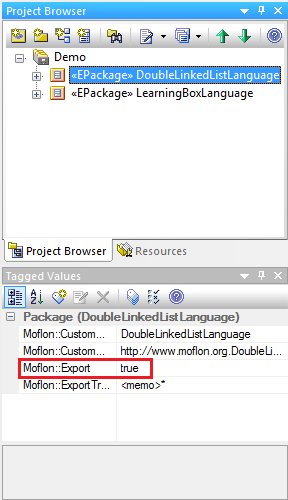
\includegraphics[width=0.5\textwidth]{pics/tricks/ignoreExportingProject/ignoreExportingProject2}
  \caption{Default TaggedValue}  
  \label{fig_ignoreExportingProject02}
\end{center}
\end{figure}



\begin{figure}[htbp]
\begin{center}
  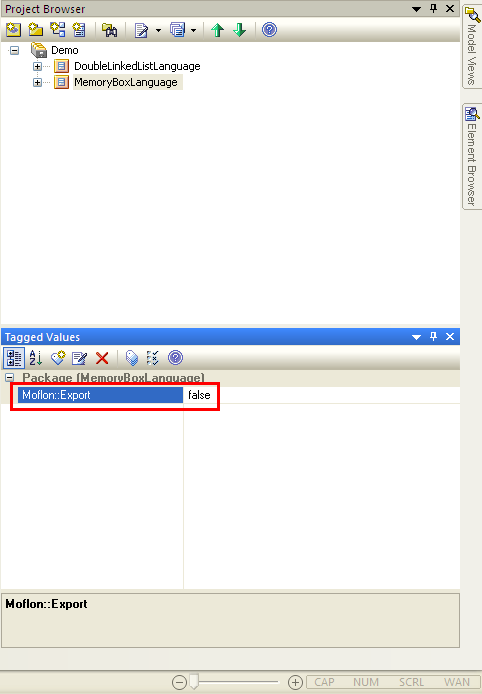
\includegraphics[width=0.5\textwidth]{pics/tricks/ignoreExportingProject/ignoreExportingProject3}
  \caption{Chaging the TaggedValue}  
  \label{fig_ignoreExportingProject03}
\end{center}
\end{figure}

\end{enumerate}


\section{Using Verbose tag to show create and destroy stereotypes} As you have already seen in previous chapters there are different colors in SDMs in 
order to distinguish between ``create'' and ``destroy''.

\begin{enumerate}
\item[$\blacktriangleright$]If you want to have a black white print of diagram 
you can set the these properties in a \emph{verbal} way. Right–click on the
diagram and select'' Extensions/extras/Set Moflon::Verbose to
true''. Now you can see \texttt{<<create>>} and \texttt{<<destroy>>} on the
links (Fig.~\ref{fig_usingVerbose01}).

\begin{figure}[htbp]
\begin{center}
  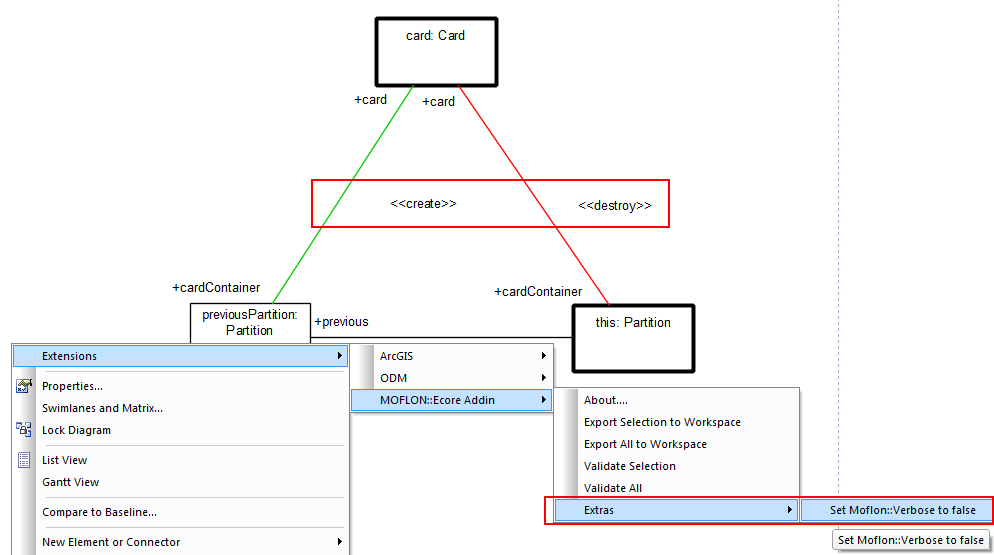
\includegraphics[width=0.5\textwidth]{pics/tricks/usingVerbose/usingVerbose1}
  \caption{Verbal change of links}  
  \label{fig_usingVerbose01}
\end{center}
\end{figure}


\item[$\blacktriangleright$]You can undo this change by selecting
``Extensions/extras/Set Moflon:: Verbose to
false'' (Fig.~\ref{fig_usingVerbose02}).

 \begin{figure}[htbp]
\begin{center}
  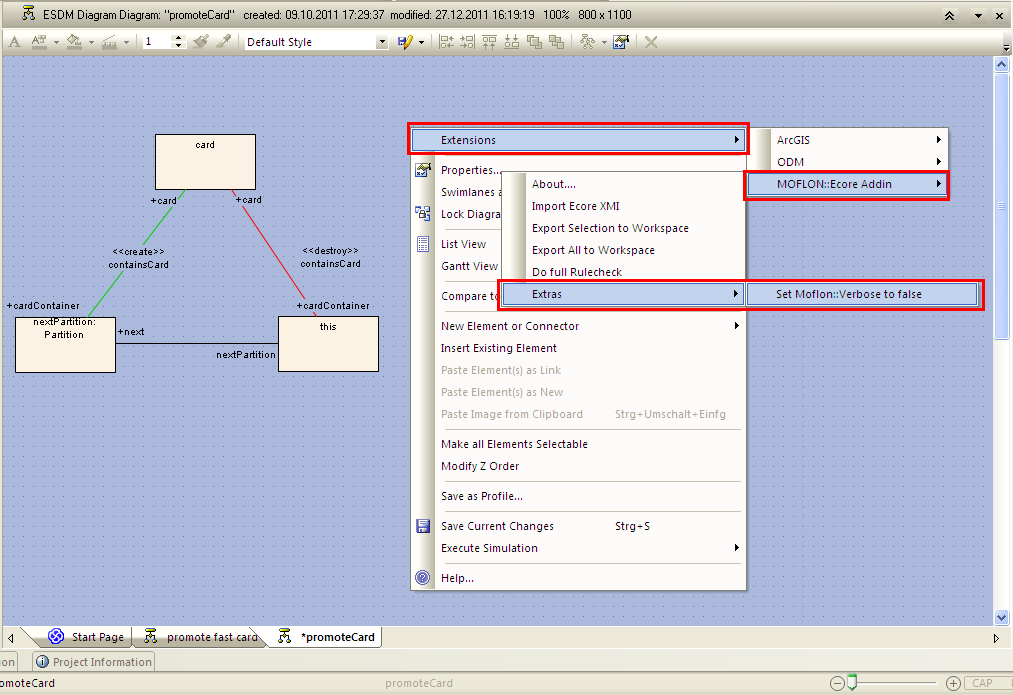
\includegraphics[width=0.5\textwidth]{pics/tricks/usingVerbose/usingVerbose2}
  \caption{Undo Verbal change of a link}  
  \label{fig_usingVerbose02}
\end{center}
\end{figure}

\end{enumerate}


\section{Copying object variables with ctrl + drag}
By holding down \texttt{Ctrl} and dragging the objects, you can copy object
variables (Fig.~\ref{fig_copy01}).You can see the new copied object in Project
Browser (Fig.~\ref{fig_copy02}).

\begin{enumerate}
\item[$\blacktriangleright$]
\begin{figure}[htbp]
\begin{center}
  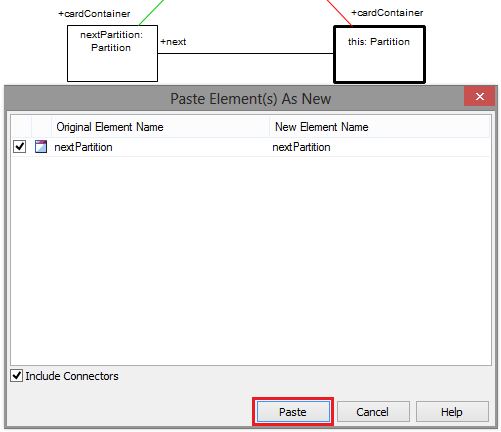
\includegraphics[width=0.5\textwidth]{pics/tricks/copy/copy1}
  \caption{Copying objects}  
  \label{fig_copy01}
\end{center}
\end{figure}


\begin{figure}[htbp]
\begin{center}
  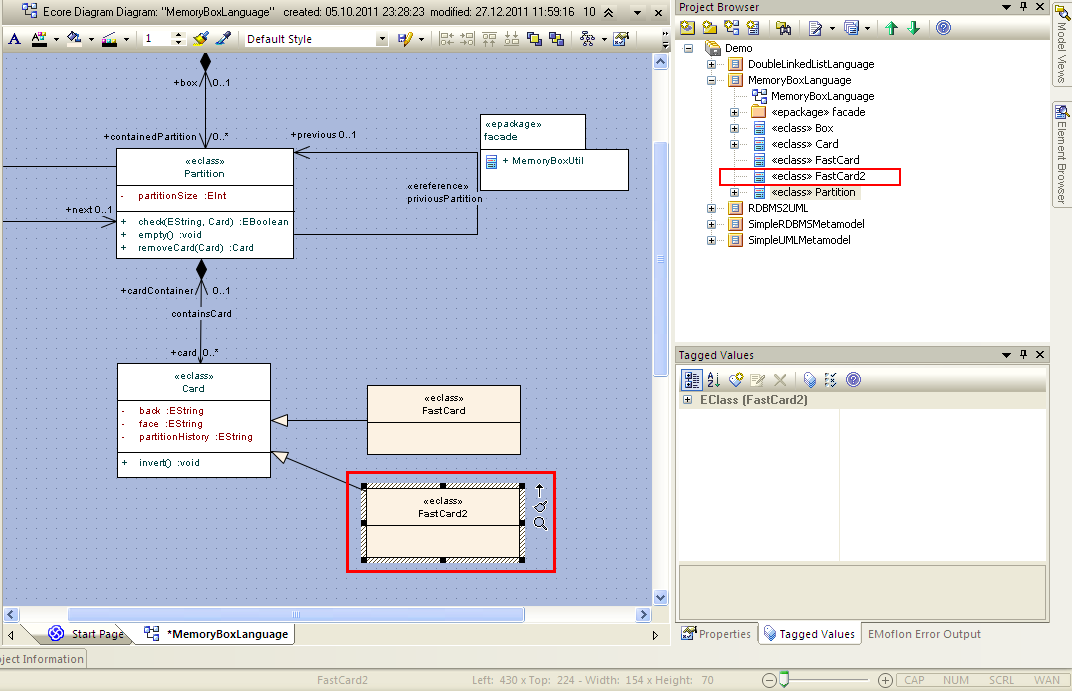
\includegraphics[width=0.5\textwidth]{pics/tricks/copy/copy2}
  \caption{Copied object in Project Browser}  
 
  \label{fig_copy02}
\end{center}
\end{figure}

\end{enumerate}


\section{Searching for Elements}
The Model Search allows you to quickly navigate and find elements within your
model.


\begin{enumerate}
\item[$\blacktriangleright$]Select ``Model Search Window'' and type the name of
element you search for (Fig.~\ref{fig_search01}). 
\begin{figure}[htbp]
\begin{center}
  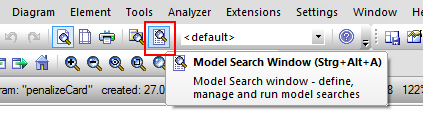
\includegraphics[width=0.5\textwidth]{pics/tricks/search/search1}
  \caption{Model Search Window}  
  \label{fig_search01}
\end{center}
\end{figure}

\item[$\blacktriangleright$]It lists each element that meets the search criteria
you specify within the ``search terms'' and ``search type'' (Fig.~\ref{fig_search02}).
\begin{figure}[htbp]
\begin{center}
  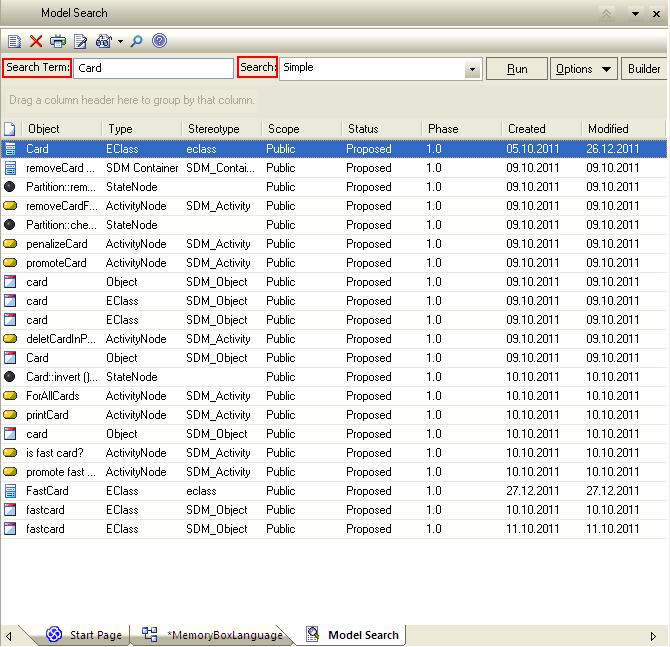
\includegraphics[width=0.5\textwidth]{pics/tricks/search/search2}
  \caption{Enter search criteria}  
  \label{fig_search02}
\end{center}
\end{figure}

\item[$\blacktriangleright$]Right-Click on each of the item and selecting ``Find
in Diagrams'' (Fig.~\ref{fig_search03}). 
\begin{figure}[htbp]
\begin{center}
  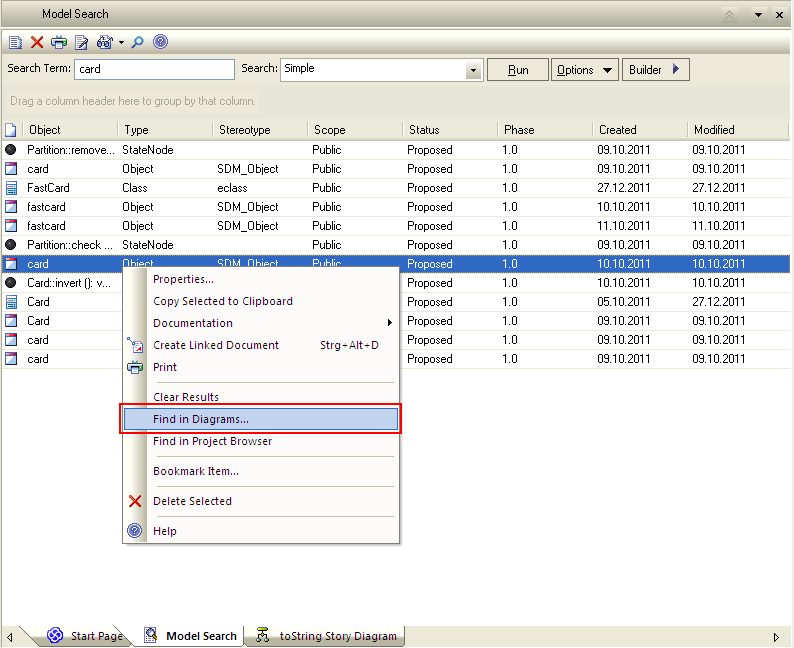
\includegraphics[width=0.5\textwidth]{pics/tricks/search/search3}
  \caption{Finding an element in diagrams}  
  \label{fig_search03}
\end{center}
\end{figure}

\item[$\blacktriangleright$]Right click on each of the item an selecting ``Find in
Project Browser'' (Fig.~\ref{fig_search04}). 
\begin{figure}[htbp]
\begin{center}
  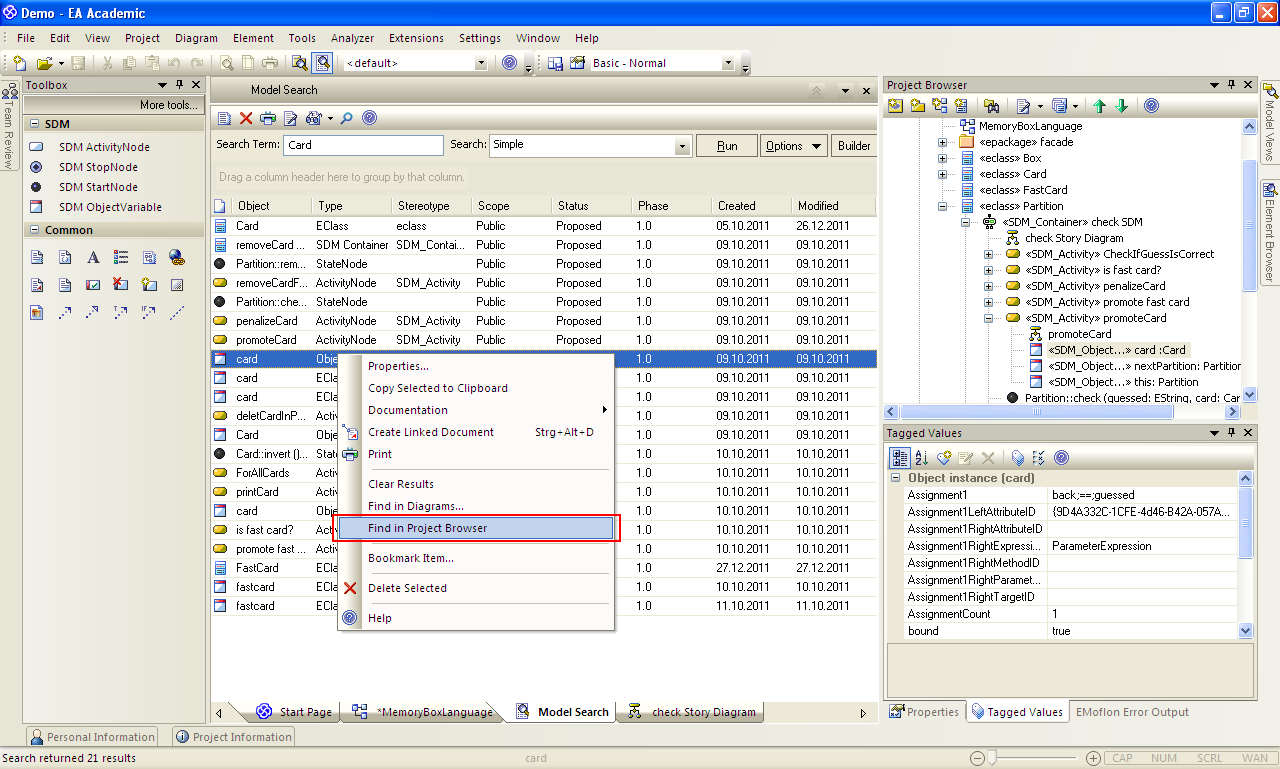
\includegraphics[width=0.5\textwidth]{pics/tricks/search/search4}
  \caption{Finding an element in Project Browser}  
  \label{fig_search04}
\end{center}
\end{figure}

\item[$\blacktriangleright$]If you want to see an specified obejct of a diagram
in the \texttt{Project Browser} , Rightclick on the object and select ``Find/In Project
Browser'' (Fig.~\ref{fig_search05}). In a similar way you can find the
corresponding class of object by Rightclick and selecting ``Find/Locate
Classifier in Project Browser'' (Fig.~\ref{fig_search06}).

\begin{figure}[htbp]
\begin{center}
  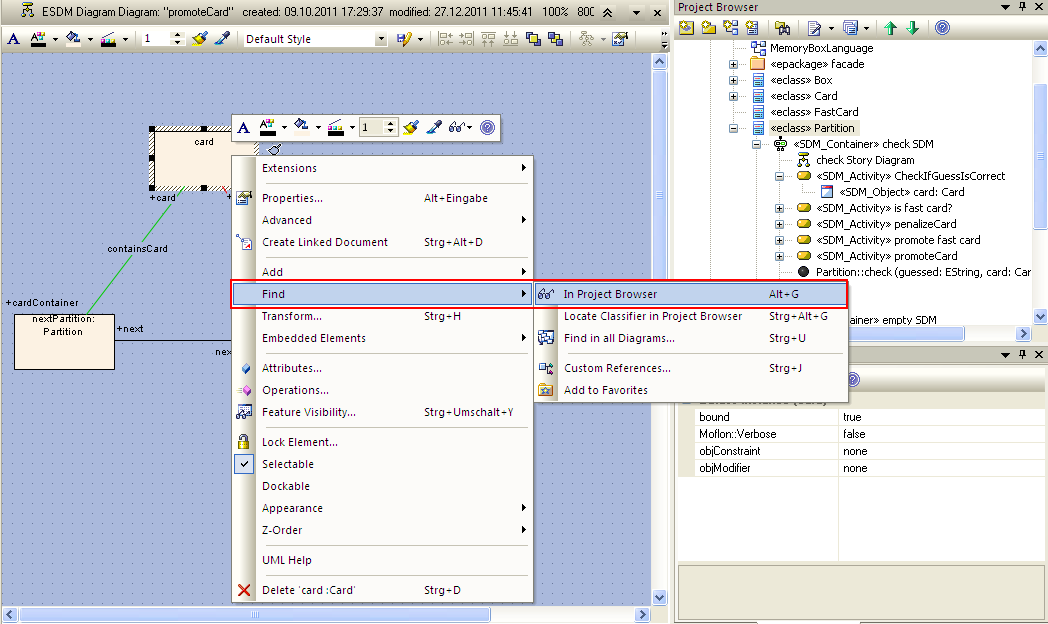
\includegraphics[width=0.5\textwidth]{pics/tricks/search/search5}
  \caption{Following an object from diagram to Projet Browser}  
  \label{fig_search05}
\end{center}
\end{figure}


\begin{figure}[htbp]
\begin{center}
  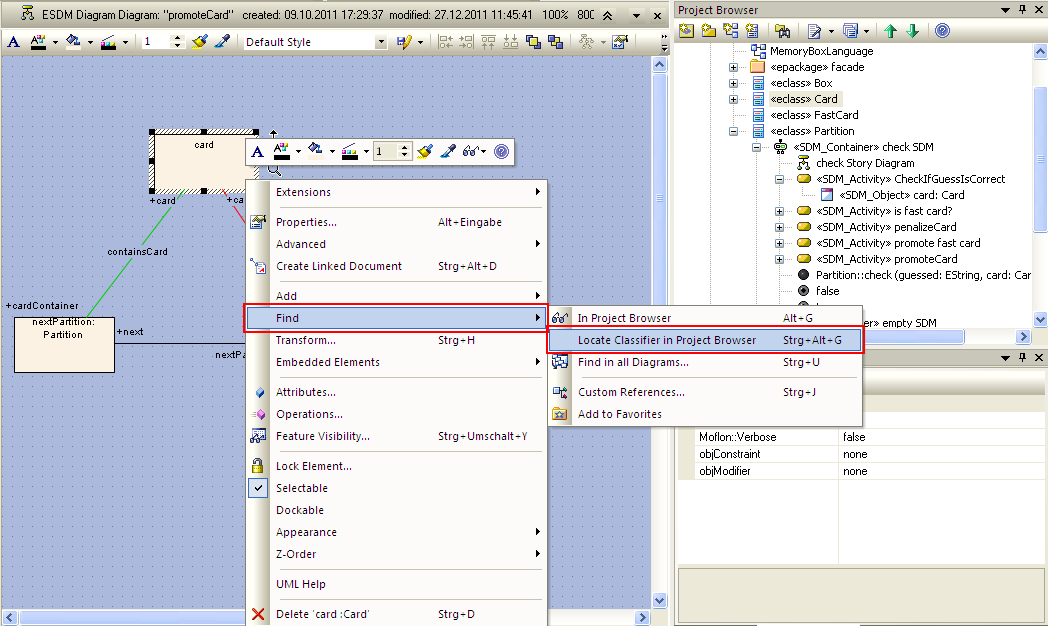
\includegraphics[width=0.5\textwidth]{pics/tricks/search/search6}
  \caption{Finding the corresponding class of an object in the diagram}  
  \label{fig_search06}
\end{center}
\end{figure}

\end{enumerate}


\section{Using multiple EAPs and migrating packages} 

\begin{enumerate}
\item[$\blacktriangleright$]If you want to migrate multiple packages between
multiple EAPs (EA Projects),You can't do it by just copy and
paste the selected packages (Fig.~\ref{fig_projectMigration00}) from/to EAPs.


\begin{figure}[htbp]
\begin{center}
  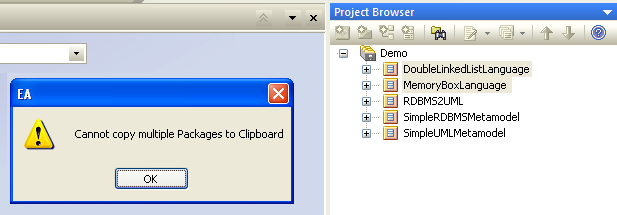
\includegraphics[width=0.5\textwidth]{pics/tricks/projectMigration/projectMigration0}
  \caption{Error message}  
  \label{fig_projectMigration00}
\end{center}
\end{figure}

\item[$\blacktriangleright$]In order to migrate multiple packages, you have to
first export the Whole model(the root node) from one EAP. Right-Click on the root
and select ``Export Model to XMI...''. In the dialogue that
pops up (Fig.~\ref{fig_projectMigration01}), enter the name and path of to be
exported file, choose \texttt{XMI 2.1} as``Export
type'' (Fig.~\ref{fig_projectMigration02}).


\begin{figure}[htbp]
\begin{center}
  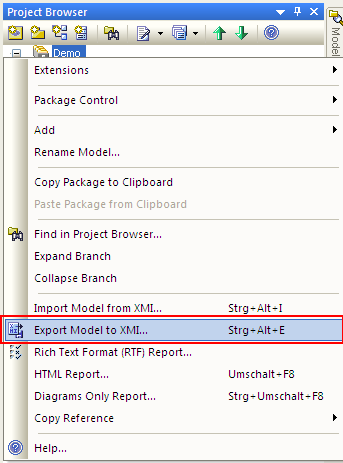
\includegraphics[width=0.5\textwidth]{pics/tricks/projectMigration/projectMigration1}
  \caption{Export the Root Model from the first EAP}  
  \label{fig_projectMigration01}
\end{center}
\end{figure}


\item[$\blacktriangleright$]Go to the other EAP, right-click on the Project
Browser and select ``Import Model from
XMI...'' (Fig.~\ref{fig_projectMigration03}). In the Dialogue that pops up, enter
the name and path of to be imported file and click on \texttt{Import} (Fig.~\ref{fig_projectMigration04}).

 \begin{figure}[htbp]
\begin{center}
  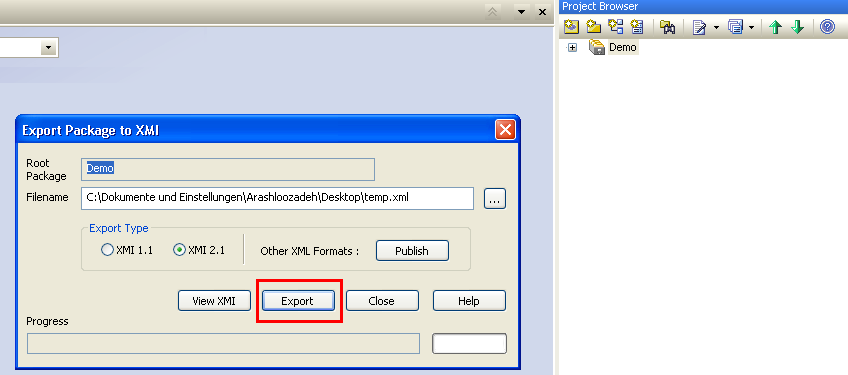
\includegraphics[width=0.5\textwidth]{pics/tricks/projectMigration/projectMigration2}
  \caption{Specify the Export file properties}  
  \label{fig_projectMigration02}
\end{center}
\end{figure}

\item[$\blacktriangleright$]In the next step you have to confirm importing of
XMI file(Fig.~\ref{fig_projectMigration05}).

\begin{figure}[htbp]
\begin{center}
  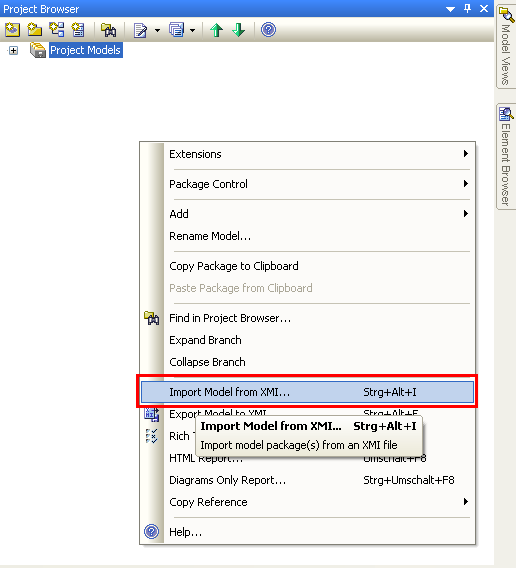
\includegraphics[width=0.5\textwidth]{pics/tricks/projectMigration/projectMigration3}
  \caption{Import the root node to the second EAP}  
  \label{fig_projectMigration03}
\end{center}
\end{figure}

\item[$\blacktriangleright$]Finally you have to specify the level of imported
file in the Project Browser either as Root Model or under selected
package (Fig.~\ref{fig_projectMigration06}).After Importing you have the whole root with all it's belonging
packages in the second EAP. Now you can delete the packages which you do not
need from the Root Model (Fig.~\ref{fig_projectMigration07}).

\begin{figure}[htbp]
\begin{center}
  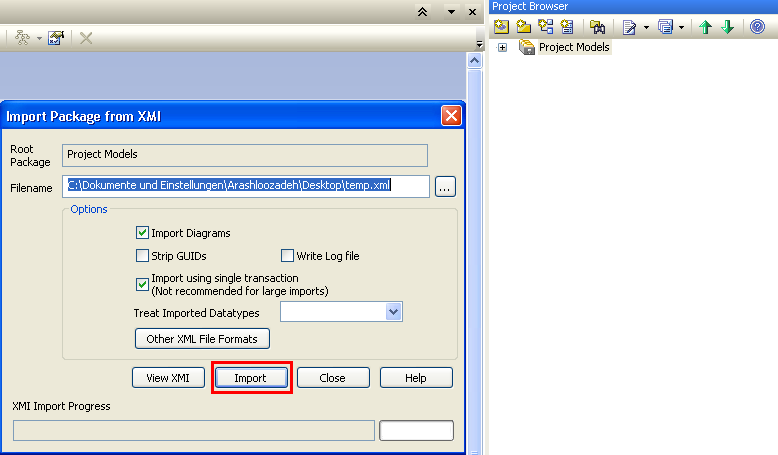
\includegraphics[width=0.5\textwidth]{pics/tricks/projectMigration/projectMigration4}
  \caption{Specify the Import file properties}  
  \label{fig_projectMigration04}
\end{center}
\end{figure}


\begin{figure}[htbp]
\begin{center}
  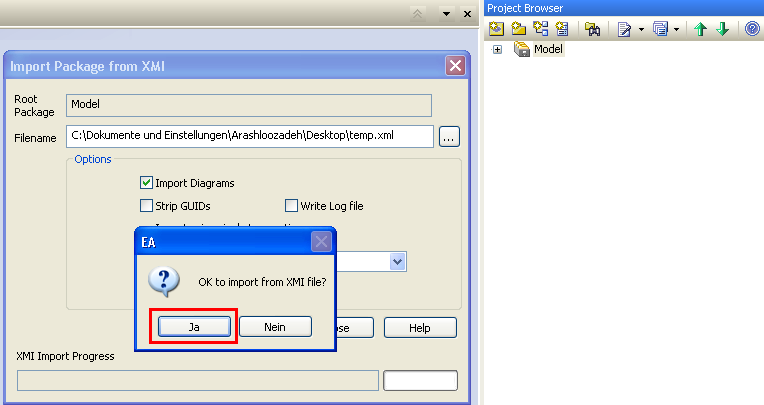
\includegraphics[width=0.5\textwidth]{pics/tricks/projectMigration/projectMigration5}
  \caption{Confirm Import}  
  \label{fig_projectMigration05}
\end{center}
\end{figure}



\begin{figure}[htbp]
\begin{center}
  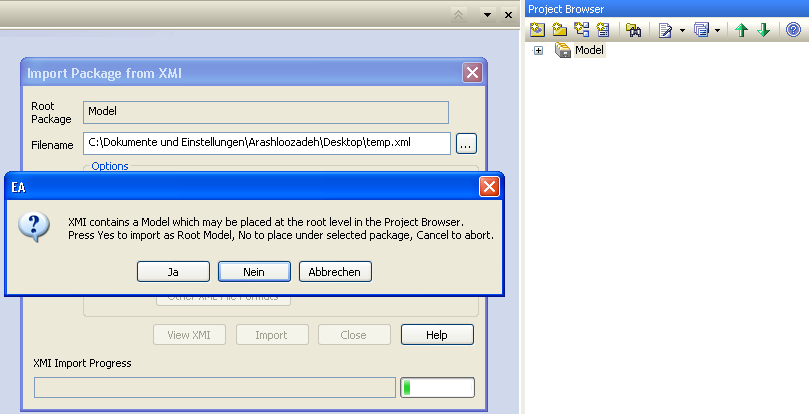
\includegraphics[width=0.5\textwidth]{pics/tricks/projectMigration/projectMigration6}
  \caption{Specify the level of imported model}  
  \label{fig_projectMigration06}
\end{center}
\end{figure}


\begin{figure}[htbp]
\begin{center}
  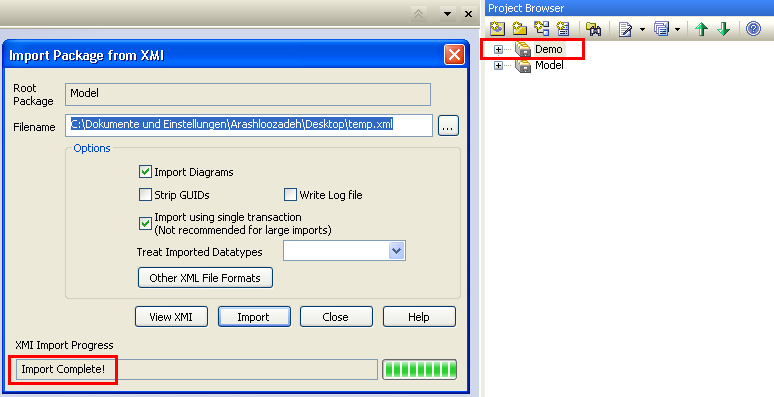
\includegraphics[width=0.5\textwidth]{pics/tricks/projectMigration/projectMigration7}
  \caption{Importing is completed}  
  \label{fig_projectMigration07}
\end{center}
\end{figure}


\end{enumerate}

